% Name: Frobenius law
% Description: The Frobenius law as string diagrams: splitting then merging across, in either direction, equals merging two strands and then splitting them again.
% Tags: string diagrams, Frobenius algebra, monoidal category, category theory

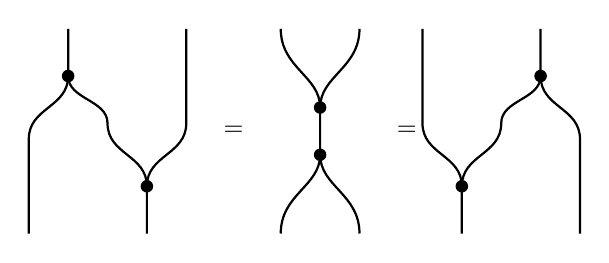
\begin{tikzpicture}[thick, every node/.style={font=\small}, dot/.style={circle, fill, inner sep=1.6pt}]
  % Left: the right strand splits, and its left half merges with the first strand
  \draw (0,0) -- (0,1.2) .. controls (0,1.6) and (0.5,1.6) .. (0.5,2) -- (0.5,2.6);
  \draw (1.5,0) -- (1.5,0.6) .. controls (1.5,1) and (1,1) .. (1,1.4) .. controls (1,1.7) and (0.5,1.7) .. (0.5,2);
  \draw (1.5,0.6) .. controls (1.5,1) and (2,1) .. (2,1.4) -- (2,2.6);
  \node[dot] at (1.5,0.6) {}; \node[dot] at (0.5,2) {};
  \node at (2.6,1.3) {$=$};
  % Middle: merge, then split
  \draw (3.2,0) .. controls (3.2,0.5) and (3.7,0.6) .. (3.7,1) (4.2,0) .. controls (4.2,0.5) and (3.7,0.6) .. (3.7,1) -- (3.7,1.6);
  \draw (3.7,1.6) .. controls (3.7,2) and (3.2,2.1) .. (3.2,2.6) (3.7,1.6) .. controls (3.7,2) and (4.2,2.1) .. (4.2,2.6);
  \node[dot] at (3.7,1) {}; \node[dot] at (3.7,1.6) {};
  \node at (4.8,1.3) {$=$};
  % Right: the mirror image of the left
  \draw (7,0) -- (7,1.2) .. controls (7,1.6) and (6.5,1.6) .. (6.5,2) -- (6.5,2.6);
  \draw (5.5,0) -- (5.5,0.6) .. controls (5.5,1) and (6,1) .. (6,1.4) .. controls (6,1.7) and (6.5,1.7) .. (6.5,2);
  \draw (5.5,0.6) .. controls (5.5,1) and (5,1) .. (5,1.4) -- (5,2.6);
  \node[dot] at (5.5,0.6) {}; \node[dot] at (6.5,2) {};
\end{tikzpicture}
